% Cross-Era Fantasy Cricket - final report (submission version).
% Format required by the course: course LaTeX template UNMODIFIED, max 4 double-column pages INCLUDING references,
% with Individual Contributions, a Generative AI Disclosure and the public GitHub link.
% The course template was not in the repository; this file uses a plain two-column article with the same sections.
% To submit: paste the body (from \begin{abstract} to the bibliography) into the course template, keep figs/ and
% refs.bib next to it, compile on Overleaf (pdflatex + bibtex) and check the page count is <= 4.
% If it runs over: drop Fig. 3 (bowler strip) first, then shrink Fig. 2.
\documentclass[10pt,twocolumn]{article}
\usepackage[a4paper,margin=0.7in,columnsep=0.25in]{geometry}
\usepackage{graphicx,booktabs,amsmath,url,microtype}
\usepackage[hidelinks]{hyperref}
\usepackage[font=small,labelfont=bf]{caption}
\setlength{\textfloatsep}{7pt plus 2pt minus 2pt}
\setlength{\floatsep}{5pt plus 2pt minus 2pt}
\setlength{\abovecaptionskip}{3pt}

\title{\vspace{-1.5em}Cross-Era Fantasy Cricket: Animating Historical Cricketers\\with Modern Motion on Free Hardware\vspace{-0.5em}}
\author{[TODO: names and IDs] \quad Course: [TODO: course code and name]}
\date{\vspace{-1.8em}}

\begin{document}
\maketitle

\begin{abstract}
We animate historical cricketers from a single archival photograph using motion from modern footage, and render the
result in the visual style of the player's era. Our main pipeline extracts whole-body pose with DWPose on a laptop CPU,
builds a pose-skeleton or depth control video, generates the clip with Wan2.1-VACE-1.3B in a headless ComfyUI on a free
Kaggle T4 GPU, retimes it to real speed and applies 1930s/1970s/1990s era filters. A $2{\times}2$ ablation (control
$\times$ reference crop) with a seed sweep shows that depth control fixes the most visible failure of skeleton control,
a lost or wrong bat, and lowers brightness flicker, while a tighter reference crop does not clearly improve likeness. We
compare against the team's skeleton-driven baseline (a rigid 3D skeleton fit driving MusePose) and explain why it fails
on fast bowling: blurred, cropped source footage and the front/back ambiguity of a skeleton, both of which a clean
clip and a depth control avoid. All outputs are labelled ``AI-generated -- academic project''.
\end{abstract}

\section{Introduction}
``Fantasy cricket'' across eras is usually a statistical exercise. We ask what such a match could \emph{look} like:
Sir Don Bradman playing a modern cover drive, or Harold Larwood bowling a modern delivery. This is reference-guided human
image animation: one photograph supplies the appearance, a driving video supplies the motion. Cricket makes it hard:
fast limb motion, a thin bat that a skeleton does not describe, other people in frame, and archival references that are
black-and-white, low resolution and often half-body. Our constraints were a laptop with a 6\,GB RTX 4050 and no paid
GPUs.

Contributions: (i) a reproducible free pipeline (laptop CPU + Kaggle T4) from a modern clip to an era-styled video;
(ii) a depth control with a \emph{target-only} mode that removes other people and preserves the bat; (iii) a controlled
ablation, including an honest negative result on reference cropping; (iv) a diagnosis of why a skeleton-driven baseline
fails on fast bowling, with measured causes.

\section{Related Work}
\textbf{Pose.} DWPose~\cite{yang2023dwpose} distils RTMPose~\cite{jiang2023rtmpose} into a 133-keypoint whole-body
estimator; BlazePose~\cite{bazarevsky2020blazepose} adds per-joint depth. \textbf{Human animation.} Animate
Anyone~\cite{hu2023animateanyone}, MagicAnimate~\cite{xu2023magicanimate} and MusePose~\cite{musepose2024} add a
reference branch to Stable Diffusion with pose or DensePose guidance; AnimateDiff~\cite{guo2023animatediff} adds a motion
module; MimicMotion~\cite{zhang2024mimicmotion} uses confidence-aware pose guidance. The proposal named
LTX-2~\cite{ltx2} and MagicAnimate. LTX-2 uses the reference only as a first frame and targets 32\,GB+ GPUs, and
MagicAnimate's code is SD1.5/DensePose-based, so AnimateDiff/MagicAnimate became the team baseline.
\textbf{Video DiTs.} Wan2.1~\cite{wan2025} is an open video diffusion-transformer family; VACE~\cite{jiang2025vace}
adds unified conditioning (reference images, pose, depth, masks), and its 1.3B variant fits a free T4.
\textbf{Depth and features.} Depth Anything V2~\cite{yang2024depthanythingv2} gives relative depth;
DINOv2~\cite{oquab2023dinov2} gives features for an identity proxy; U$^2$-Net~\cite{qin2020u2net} (rembg) removes
backgrounds.

\begin{figure*}[t]
  \centering
  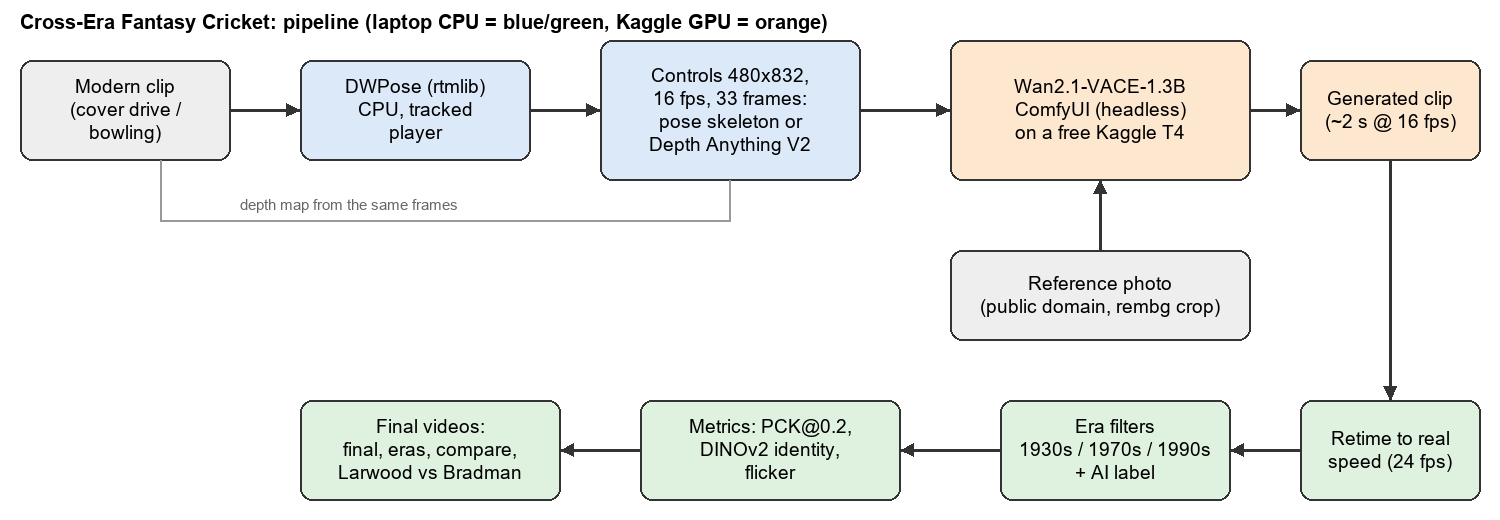
\includegraphics[width=0.70\textwidth]{figs/pipeline.png}
  \caption{Main pipeline. Laptop CPU stages in blue/green, the Kaggle T4 stage in orange.}
  \label{fig:pipeline}
\end{figure*}

\section{Method}
\textbf{Motion extraction.} rtmlib's YOLOX detector and DWPose-l ($384{\times}288$) run on CPU. The player is selected by
a box on frame~0 and followed by best-IoU tracking (umpire, non-striker and fielders share the frame). Keypoints below
confidence 0.3 are masked, gaps of up to 4 frames interpolated, and trajectories smoothed (Savitzky--Golay, window 7).
We resample to 33 frames at 16\,fps on a $480{\times}832$ canvas with one global scale and offset (body ${\approx}85\%$
of the height, 8\% top margin so a raised bowling hand stays in frame).

\textbf{Controls.} \emph{Skeleton}: OpenPose-style render (body, hands, face) on black. \emph{Depth}: Depth Anything V2
Small on the same frames, warped with the \emph{same} affine, normalised with one global min/max over the clip (no
flicker), near = bright; the head is flattened inside the silhouette so a modern helmet does not override the face.
\emph{Target-only} (bowler): a rembg person mask restricted to blobs containing the player's keypoints and a capsule
around his skeleton, so fielders become flat background.

\textbf{Reference and generation.} rembg removes the photo background; the \emph{tight crop} fills ${\approx}90\%$ of
the canvas, the \emph{padded} variant letterboxes the photo. Wan2.1-VACE-1.3B (fp16 DiT, fp8 UMT5 text encoder, fp32 VAE;
the T4 has no bf16) runs in ComfyUI driven headlessly through its API: 20 steps, CFG 5, \texttt{uni\_pc}, shift 8.
A 33-frame run takes ${\approx}$520\,s at a 14.9\,GB peak, so 33 frames is the T4 limit (the 6\,GB laptop GPU cannot run
it). The prompt describes 1930s kit; the negative prompt lists failure modes (extra balls, two bats, logos; for the bowler
also bat, hat, suit, cigarette).

\textbf{Post-processing.} The batter's 33 frames cover 5.6\,s of source, so we retime to real speed at 24\,fps with
frame blending (motion-compensated interpolation tore the thin bat). Seeded era filters (Table~\ref{tab:eras}) keep the
duration and burn in the ``AI-generated'' label.

\textbf{Metrics.} \emph{PCK@0.2}: DWPose on the output vs the control keypoints (17 joints, $0.2\times$ torso length).
\emph{Identity}: DINOv2-small cosine between grayscale person crops and the tight (``crop'') or original (``orig'')
reference. \emph{Flicker}: std of per-frame mean brightness (B.std) and mean frame difference (F.diff).

\section{Results}
\begin{table}[t]
\centering\small
\setlength{\tabcolsep}{3.0pt}
\begin{tabular}{lllccccc}
\toprule
Run & Ctrl & Ref & PCK & ID$_\text{crop}$ & ID$_\text{orig}$ & B.std & F.diff\\
\midrule
A  & skel  & pad  & 0.934 & 0.205 & 0.158 & 2.27 & 10.10\\
B  & depth & pad  & 0.997 & 0.223 & 0.291 & 1.63 & 11.43\\
C  & skel  & crop & 0.969 & 0.172 & 0.130 & 2.49 & 10.62\\
D1 & depth & crop & 0.983 & 0.206 & 0.207 & 1.98 & 10.26\\
D2 & depth & crop & 0.900 & 0.230 & 0.227 & 1.49 & 10.97\\
D3 & depth & crop & 0.979 & 0.165 & 0.156 & 2.06 & 11.90\\
D4 & depth & crop & 0.990 & 0.302 & 0.305 & 1.25 & 10.40\\
\midrule
F1 & depth & crop & 0.904 & 0.217 & 0.175 & 1.65 & 11.93\\
F2 & depth & crop & 0.882 & 0.203 & 0.195 & 3.78 & 9.17\\
\midrule
L1 & depth$^\dagger$ & crop & 0.788 & 0.124 & 0.108 & 4.26 & 12.17\\
L2 & depth$^\dagger$ & crop & 0.851 & 0.092 & 0.102 & 4.93 & 15.42\\
L3 & depth$^\dagger$ & crop & 0.801 & 0.125 & 0.086 & 1.81 & 11.06\\
\bottomrule
\end{tabular}
\caption{VACE runs. A--D: 17 frames, seed 42 except D2--D4 (7/123/2024). F1 (cap) / F2 (bare-headed): final batter,
33 frames. L1--L3: Larwood bowling, 33 frames, seeds 42/7/2024, $^\dagger$target-only depth.}
\label{tab:ablation}
\end{table}

\begin{figure*}[t]
  \centering
  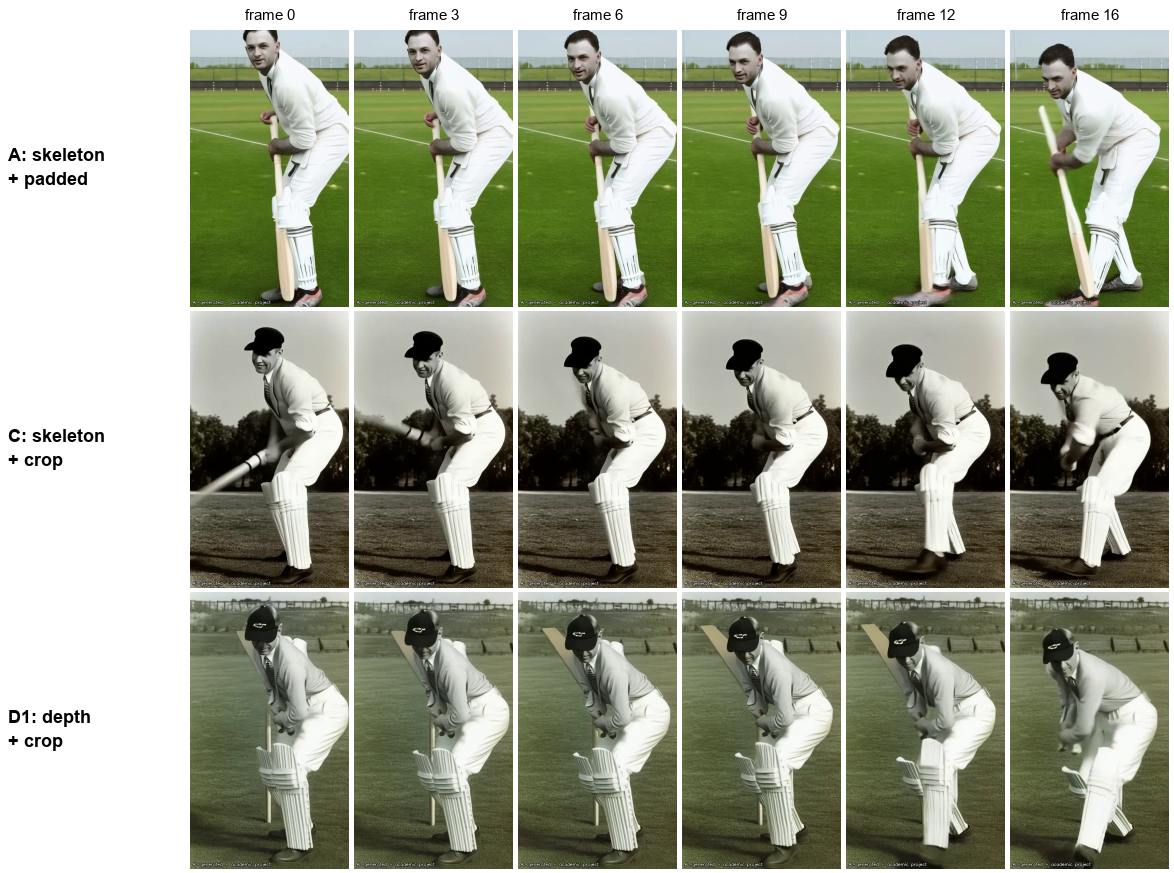
\includegraphics[width=0.56\textwidth]{figs/ablation_strip.png}\hfill
  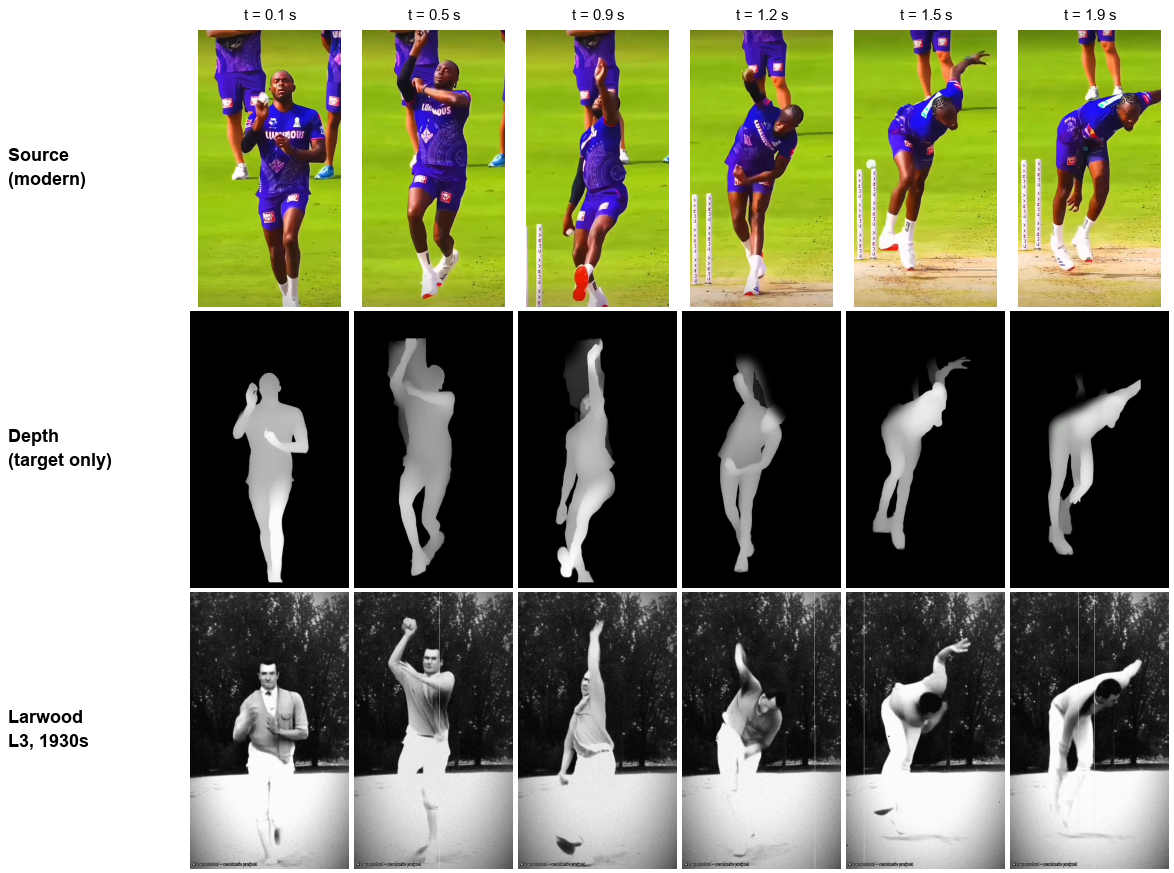
\includegraphics[width=0.42\textwidth]{figs/bowler_strip.png}
  \caption{Left: ablation outputs. With the skeleton (A, C) the bat is lost or wrong; with depth (D1) one bat is held
  for the whole clip. Right: Larwood bowling (L3) from the target-only depth control.}
  \label{fig:strips}
\end{figure*}

\textbf{Depth fixed the bat.} Every depth run (B, D1--D4) holds one proper bat for the whole clip; both skeleton runs
(A, C) lose it (Fig.~\ref{fig:strips}), because a skeleton carries no bat information. Motion fidelity stays high
(PCK 0.90--1.00). \textbf{Flicker.} Depth lowered brightness flicker (mean B.std 2.38 skeleton vs 1.68 depth); frame
difference did not drop (10.36 vs 10.99), plausibly because the bat swings through a fuller arc.
\textbf{Reference crop: no clear gain.} With control and seed fixed, padded$\rightarrow$crop changes identity by
$-0.017$/$-0.084$ (depth, B$\rightarrow$D1) and $-0.034$ (skeleton, A$\rightarrow$C); a dark cap hides the face in the
crop runs. \textbf{Seed dominates}: across D1--D4 identity spans 0.137--0.149, several times the reference effect, so
single-seed likeness comparisons are inconclusive, whereas the bat result held in 5/5 depth runs and failed in 2/2
skeleton runs. \textbf{Finals}: F1 and F2 are close numerically; we chose F1 (cap) visually.
\textbf{Bowler}: all three Larwood runs are bare-headed with no fedora, suit or cigarette (the negative prompt overrode
the 1929 reference clothing) and show no extra people. PCK is lower (0.79--0.85) because the overarm action is the
fastest, most blurred motion. We chose L3 (most 1930s kit, lowest flicker), shown at $2{\times}$ slow motion.
\textbf{Era filters} keep the motion (Table~\ref{tab:eras}): batter PCK drops by at most 0.08, the bowling arm by up to
0.12; the 1930s look deliberately adds flicker and texture, the 1970s/1990s filters lower the warping error.

\begin{table}[t]
\centering\small
\setlength{\tabcolsep}{2.4pt}
\begin{tabular}{llcc}
\toprule
Preset & Look & PCK bat/bowl & Warp bat/bowl\\
\midrule
raw & VACE output, 16\,fps & 0.904 / 0.801 & 5.72 / 3.40\\
1930s & 18\,fps, gray, grain, weave, flicker & 0.870 / 0.698 & 9.81 / 9.91\\
1970s & 25\,fps, desat., chrom.\ aberr., scanlines & 0.829 / 0.684 & 4.06 / 3.08\\
1990s & 25\,fps, mild colour, chroma bleed & 0.897 / 0.774 & 3.27 / 2.65\\
\bottomrule
\end{tabular}
\caption{Era presets on Bradman F1 / Larwood L3. Warp: Farneback warping error (lower = smoother).}
\label{tab:eras}
\end{table}

\section{Comparison: Skeleton-Driven Baseline}
The integration branch drove MusePose~\cite{musepose2024} (SD1.5 with a pose guider, 30 steps, $560{\times}632$, Kaggle
T4) with a skeleton only. To make that skeleton as clean as possible it fits one rigid 3D skeleton per clip: DWPose and
MediaPipe~\cite{bazarevsky2020blazepose} detections, background camera tracking for a fixed ground, constant bone
lengths (max error $<0.6$\,px), planted feet, smoothness of every bone vector and a rigid bat. This removed the
skeleton's own glitches: joint acceleration p99 fell from 318 to 10\,px/frame$^2$ on the bowling clip, bat-length change
per frame (p99) from 53\% to 0.1\%, and no joint is ever missing. The players are placed into scenes (Bradman on the
clip's own pitch, McGrath in his photo) and the bat and ball are composited after generation.

\begin{table}[t]
\centering\small
\setlength{\tabcolsep}{2.2pt}
\begin{tabular}{lcccc}
\toprule
MusePose run & PCK@0.1 & view-tol. & merged & mirrored\\
\midrule
Bradman, cover drive & 0.963 & -- & 0.7\% & --\\
McGrath, 1st 3D skeleton & 0.723 & 0.884 & 21\% & 40\%\\
McGrath, legs fixed & 0.638 & 0.877 & 18\% & 60\%\\
\bottomrule
\end{tabular}
\caption{Baseline results. PCK@0.1 (of the body box) is stricter than PCK@0.2 of the torso above. View-tolerant PCK
allows a left/right-mirrored detection per frame; ``mirrored'': share of frames detected mirrored.}
\label{tab:baseline}
\end{table}

Batting worked (Table~\ref{tab:baseline}), but bowling did not, and the side-by-side with VACE shows why.
\textbf{(1) Source footage.} The bowling source was a dark, side-on slow-motion screen recording: the arm is blurred
from the gather onwards and the feet leave the frame from the delivery stride, so both detectors miss or mislocate the
joints there. The blurred arm had to be hand-keyframed and the unseen legs borrowed from another bowler's clip; when the
legs were first inferred from anatomy alone they crossed in 45 of 100 frames. The VACE bowler clip is sharp,
front-on and fully in frame (median keypoint confidence 0.77, no lost frames). \textbf{(2) Skeleton vs depth.} A
skeleton does not say which limb is in front. On a side-on body MusePose rendered, and DWPose read, the bowler mirrored in
up to 60\% of frames, which merges and swaps limbs; strict PCK falls to 0.64 while view-tolerant PCK stays at 0.88. A
depth silhouette fixes front/back and the body outline, so VACE could not flip the body. \textbf{(3) Facing.} McGrath's
photo shows him bowling to the right, the source bowler runs left; a Procrustes test on the 3D skeleton matched the photo
at 59\,px only when viewed from the other side (156\,px as filmed). VACE's front-on clip and front-on Larwood photo
agree. \textbf{(4) Mapping.} Retargeting bone lengths to the reference and placing the skeleton into the photo adds error
(91\,px alignment); VACE needs no retargeting. Post-processing of the baseline (512$\times$512 crop to $\le$100 frames,
colours matched to the photo, temporal stabilisation, each step re-scored and kept only if no score fell) raised a colour
realism score from 64 to 85 without changing motion scores, but cannot fix the motion causes above.

\section{Limitations and Ethics}
\textbf{Limitations.} Likeness is weak: identity scores are low in absolute terms, and whole-body DINOv2 crops also
measure clothing and pose, so they rank runs rather than measure likeness. The depth map keeps the modern helmet's
outline, so a dark cap often hides the face. Clips are short (2--5.6\,s, 33 frames is the T4 limit), single-player and
single-seed for the finals; bowler and batter are generated separately and cut together. The 3D skeleton's side views
are inferred from one camera.
\textbf{Ethics.} The videos show real, deceased public figures in actions they never performed. Every generated frame
carries a burned-in ``AI-generated -- academic project'' label; the work is for academic use only. Reference photos are
public domain (Larwood: National Library of Australia, Fairfax glass plate, 1929, nla.obj-161865715; Bradman: [TODO:
source]). Modern clips are used only to extract motion, are not redistributed, and their overlays are blurred in figures.
MusePose weights are licensed for non-commercial research only.

\section{Individual Contributions}
[TODO: confirm with the team.] \textbf{Student 1} [TODO name]: pose/motion engine (tracking, DWPose, DensePose,
smoothing). \textbf{Student 2, Ahaan}: AnimateDiff/MagicAnimate generation engine (team baseline).
\textbf{Student 3, Krishav}: VACE pipeline (depth and target-only controls, Kaggle notebook, retiming, final videos),
ablation, bowler clip, era styling and evaluation. \textbf{Pranahv}: integration pipeline, rigid 3D skeleton fit and
MusePose baseline, scene compositing, post-processing and its step-wise evaluation.

\section{Generative AI Disclosure}
We used Claude (Anthropic) for background research, code (pipeline scripts, the Kaggle notebook, the 3D skeleton fit)
and drafting this report. All code was run and tested by us, all numbers were checked against our own runs, and the
design decisions and conclusions are ours.

\textbf{Code:} \url{https://github.com/krishavgoyal/Cross_Era_Fantasy_Cricket} (public).

\small
\bibliographystyle{ieeetr}
\bibliography{refs}
\end{document}
